\chapter{Experimentación y Resultados}
    Aquí se presentaran los resultados del \textbf{Análisis a Priori y Posteriori} del algoritmo del granjero con Greedy
    
\section{Algoritmo: Granjero Greedy}
El algoritmo fue ejecutado en el lenguaje de programación \textbf{Python} en un entorno de \textbf{Linux}. A continuación se muestra el análisis de priori y posteriori. 
    \subsection{Análisis a Priori}
        La figura \ref{fig:priori} presenta el análisis a priori realizado sobre el pseudocódigo del algoritmo de Granjero de Greedy. Concluyendo que el algoritmo presenta \(T(n) = \theta(n)\)
        %\(f(n) = O(n)\)
        
        \begin{figure}[htp!]
            \centering
            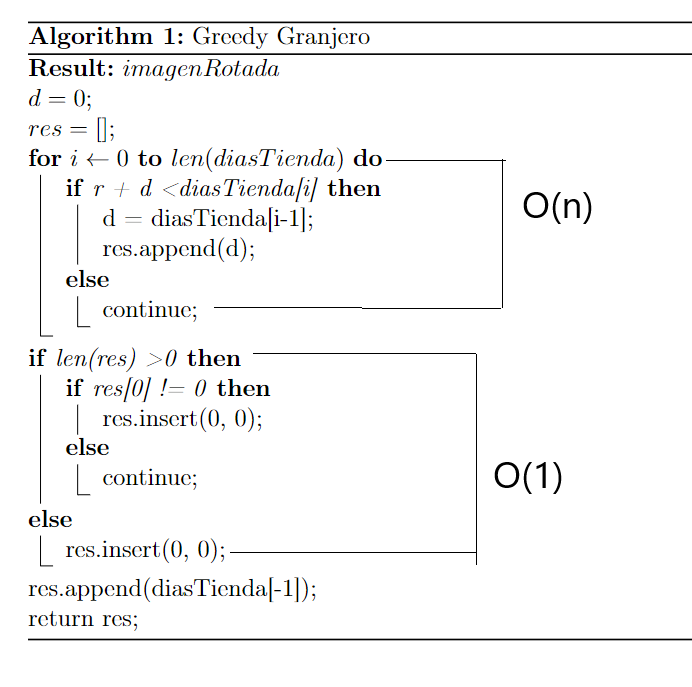
\includegraphics[width=0.5 \textwidth]{Images/A_Priori/priori.png}
            \caption{Análisis a Priori: Granjero Greedy}
            \label{fig:priori}
        \end{figure}
    
    \newpage    
    \subsection{Análisis a Posteriori}
        En el análisis posteriori se verifica que el análisis a priori demostró que la complejidad del peor caso es \(T(n) = \theta(n)\). En la figura \ref{fig:posteriori1} se muestra la función que acota al peor caso (línea verde) junto con los puntos que demuestran la complejidad del algoritmo funcionando de manera aleatoria.
        \begin{figure}[htp!]
            \centering
            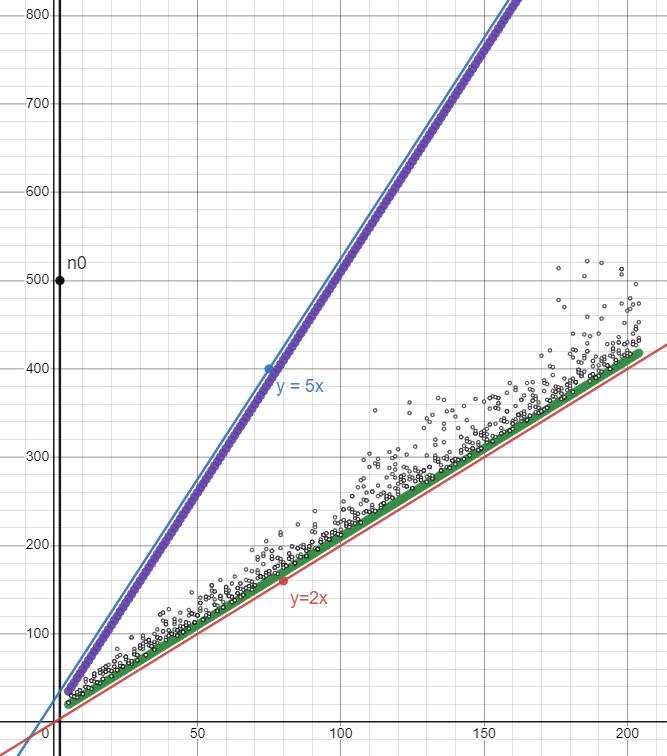
\includegraphics[width=1 \textwidth]{Images/A_Posteriori/posteriori.png}  
            \caption{Análisis a Posteriori: Granjero Greedy}
            \label{fig:posteriori1}
        \end{figure}
    
    
    
    \newpage
    \section{Pantallas de Ejecución del Algoritmo}
    Se muestra en la figura \ref{fig:terminal} la ejecución del algoritmo, demostrando la velocidad del algoritmo al ejecutar 200 casos.
    
        \begin{figure}[htp!]
            \centering
            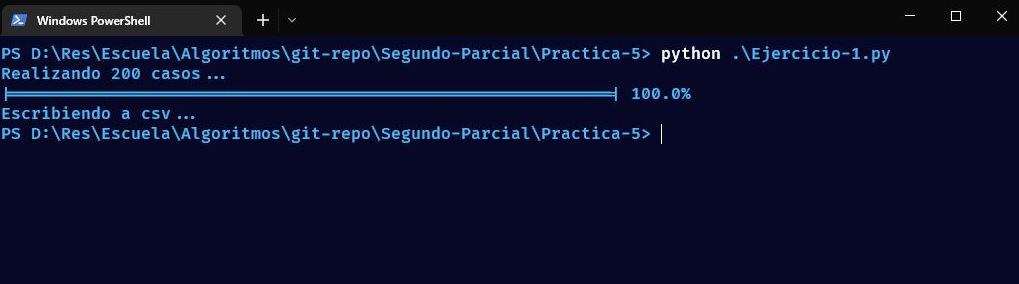
\includegraphics[width=0.8 \textwidth]{Images/Pantallas/terminal.png}  
            \caption{Ejecución de Granjero Greedy}
            \label{fig:terminal}
        \end{figure}
    